\section{Introduction}

As mobile users increasingly grow to the largest portion of internet users \cite{Rep:Marketshare}, it is important to keep in mind that these consumers of web based applications have different constraints then their personal computer counterparts. One important constraint is the limited battery life of a mobile device \cite{Rep:Batt}.

It has been shown that poor energy usage of mobile application contributes to user's negative evaluation, and may even lead to abandonment \cite{WEBSITE:2}. Considering the large market share of mobile users, this can affect revenues generated by businesses relying on these applications. This insight can be extended to web applications(web apps) which attempt to produce a native app-like experience in order to fulfill user's growing demand of functionality on web pages, while meeting a developer's requirement of portability across platforms.

Despite of the constraints presented by mobile devices, developers continue to push web technologies to deliver higher functionality while managing performance \cite{Rep:State}. Web apps that have a perceived poor performance affect profits and can lead to user abandonment. The BBC lost an additional 10\% of users for every additional second their site took to load \cite{Web:bbc}. Improving the perceived performance is crucial for increasing conversion. Pinterest rebuilt their pages for the sake of performance, realizing a 40\% reduction in perceived wait times, which increased both search engine traffic and sign-ups by 15\% \cite{Web:pinterest}.

To this end, developers have access to tools that help them assess their web app's performance and to guide the adoption of development best practices. Unlike quality requirements such as performance, 'best practices' and development guidelines provided by higher level measurement tools are lacking when it comes to energy efficiency. According to researchers, Application layer research on energy consumption can empower developers to participate in energy conscious development; but, in the context of their research, they identified a knowledge gap and limited tooling that prevented proper assessment of their application \cite{Rep:EnEf}. Without these resources, the energy mismanagement that could be introduced in the development cycle may be overlooked.

In contrast, there exist many performance bench-marking tools which help to close the knowledge gap and make performance improvements more accessible. Lighthouse is one of many bench-marking tools that attempt to make performance auditing more accessible to developers \cite{Web:Lighthouse}.

As a tool, Lighthouse, makes assessments according to the RAIL performance model, which establishes goals based on human perception \cite{Web:Rail}. Human perception in the RAIL model relates to how an application handles four key actions: the response time to a user's input, the rendering performance for animations, optimal idle-time utilization for the sake of responsiveness, and load impact on a web app. Based on the described model, Fig \ref{fig:Lighthouse} shows the metrics Lighthouse uses to score a web app:

\textit{First Contentful Paint} marks the point, when the browser renders the first bit of content and \textit{First Meaningful Paint} marks the point when the page shows its primary content. These metrics provide feedback for users that the page is actually loading. \textit{Time to interactive} measures how long it takes a page to display "useful" content, and the page responds to user interaction within 50 milliseconds.

These metrics are weighed together and ranked in a log-normal distribution of web apps in order to give a score from 0-100.

\begin{figure}[H]
  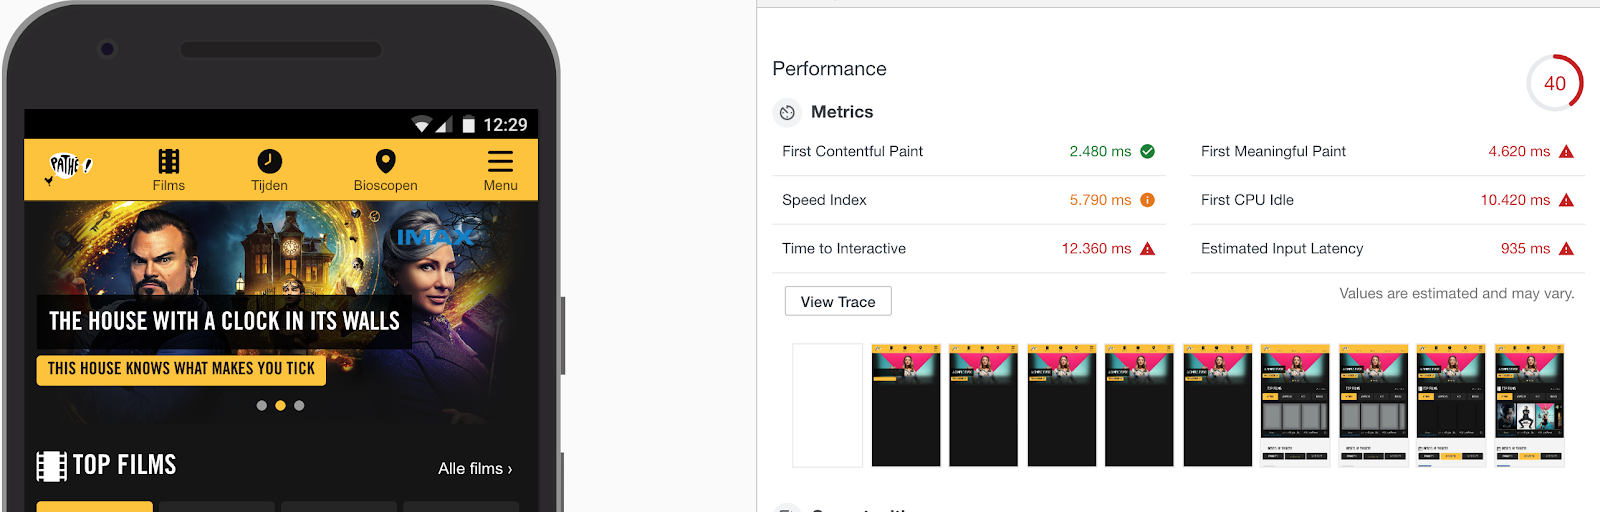
\includegraphics[width=\linewidth]{./Images/lighthousescore.png}
  \caption{Pathe.nl Lighthouse performance audit}
  \label{fig:Lighthouse}
\end{figure}

Energy consumption is overlooked in this assessment. While Web optimizations or any changes to the Web ecosystem are often studied in terms of performance, their effect on energy is not easy to measure. 

The purpose of this research is to analyze if there is a correlation between energy consumption of a web application and its measured performance, and if so, to what extent. A correlation between a high measured performance by these tools and higher energy consumption implies that tools such as these can help guide not only the performance, but also help developers take responsibility for the energy consumption of their web applications.

On the other hand, if there is no correlation, developers can employ this knowledge and use other tools to measure the energy consumption of their application, or even expand Lighthouse to also include an energy consumption meter.
\newline


